\documentclass[11pt, oneside]{amsart}

\usepackage{amsmath}
\usepackage{amssymb}

\usepackage{color}
\usepackage{dcolumn}
\usepackage{float}
\usepackage{graphicx}
\usepackage[latin9]{inputenc}
\usepackage{multirow}
\usepackage{rotating}
\usepackage{subfigure}
\usepackage{psfrag}
\usepackage{tabularx}
\usepackage[hyphens]{url}
\usepackage{wrapfig}
\usepackage{framed,color}
\usepackage{fancybox}
\usepackage{verbatim}

\usepackage[bookmarks, bookmarksopen, bookmarksnumbered]{hyperref}
\usepackage[all]{hypcap}
\urlstyle{rm}

\definecolor{orange}{rgb}{1.0,0.3,0.0}
\definecolor{violet}{rgb}{0.75,0,1}
\definecolor{darkgreen}{rgb}{0,0.6,0}
\definecolor{cyan}{rgb}{0.2,0.7,0.7}
\definecolor{blueish}{rgb}{0.2,0.2,0.8}

\definecolor{shadecolor}{rgb}{0.9,0.9,0.9}

\renewcommand{\thefootnote}{\fnsymbol{footnote}}

\newcommand{\todo}[1]{{\color{blue}$\blacksquare$~\textsf{[TODO: #1]}}}
\newcommand{\huttonnote}[1]{ {\textcolor{magenta}    { ***Eric:      #1 }}}

\DeclareRobustCommand{\csdms}{\textsc{csdms}}
\DeclareRobustCommand{\doi}{\textsc{doi}}
\DeclareRobustCommand{\bmi}{\textsc{bmi}}
\DeclareRobustCommand{\wmt}{\textsc{wmt}}

% Don't use tt font for urls
\urlstyle{rm}

\begin{document}

\title[]{Building Sustainable Software - The CSDMS Approach}

\author{
  Eric W. H. Hutton$^{\dag}$,
  Mark D. Piper$^{\dag}$,
  Scott D. Peckham$^{\dag}$,
  Irina Overeem$^{\dag}$,
  Albert J. Kettner$^{\dag}$,
  James P. M. Syvitski$^{\dag}$,
}

\thanks{{}$^{\dag}$Community Surface Dynamics Modeling System, University of
Colorado}

\begin{abstract}

\csdms{}, The Community Surface Dynamics Modeling System, is an NSF funded
project whose focus is to aid a diverse community of earth and ocean system
model \emph{users} and \emph{developers} to use and create robust software
quickly.  To this end, \csdms{} develops, integrates, archives and disseminates
earth-system models and tools to an international (67 country) community
with the goal of building the set of tools necessary to model
earth surface processes. Modelers use \csdms{} for access to over two hundred open
source surface-dynamics models and tools, as well as model metadata. Such a
model repository increases model transparency and helps eliminate
duplication by presenting the current state of community modeling efforts.
To increase software sustainability, composability and interoperability,
\csdms{} promotes standards that define common modeling interfaces, semantic
mediation between models, and model metadata. Through online resources and
workshops, \csdms{} promotes software engineering best practices, which are
less familiar to many within our community. For example,
version control, unit testing, continuous integration, test-driven
development, and well-written \emph{clean code} are all topics of the
educational mission of \csdms{}.

\end{abstract}

\maketitle

\section{The Community Surface Dynamics Modeling System}

The mission of the Community Surface Dynamics Modeling System (\csdms{})
~\cite{peckham2012component} is to help move a diverse modeling community toward
common goals and standards. This effort involves creating:
\begin{itemize}
  \item a repository of source code and metadata for open-source models and
    tools (Section~\ref{sec:organizing})
  \item reusable plug-and-play model components and a framework
        within which they can be coupled to create new models
        (Section~\ref{sec:reusable})
  \item an \emph{efficient} and \emph{open} modeling community through
        standards (Section ~\ref{sec:standards}),
        communication and education (Section~\ref{sec:education})
\end{itemize}

In building a modeling framework, \csdms{} has leveraged
several existing, well-established and open-source software tools. For example,
\csdms{} uses tools from the Common Component Architecture (CCA)
~\cite{armstrong1999toward} toolchain: \emph{Babel}, and \emph{Bocca}. Babel
provides interoperability between components
written in different languages; it currently supports C, C++, Fortran, Java,
and Python. Bocca helps with creating CCA-compliant components and managing CCA
component projects.

\csdms{} has developed innovative model/component interfaces that promote
model reuse and interoperability,
including the Basic Model Interface (\bmi{} - Section~\ref{sec:bmi}), which
uses
the \csdms{} Standard Names (Section~\ref{sec:standardnames}) and a framework
within which models can be coupled and enhanced with a set of \bmi{}-compatible
service components.
The \csdms{} Web Modeling Tool (\wmt{} - Section~\ref{sec:wmt}) is a
web-based application that provides an interface to this
framework.
It allows users to compose new models by connecting and
configuring components in a simple, browser-based graphical interface.
Further, it provides a standardized interface to standalone models;
once a user understands how to run a model in \wmt{},
they can run any model in \wmt{}.

\begin{comment}
In order to realize the full power and benefits of component-based modeling, a
modeling framework like \csdms{} needs an efficient mechanism to convert as many
open-source models as possible to reusable plug-and-play components. Since this
necessarily requires some involvement from each model's developer (\emph{who,
likely, is not paid to do this}), this mechanism must require minimal effort
and the benefit to the developer should be clear.
In the first few years of the \csdms{} project, we worked directly with model
developers and conducted one-on-one interviews to hear their concerns and
complaints about early designs and other frameworks. In addition to being easy
to implement, the following requirements of a model wrapping procedure became
clear:
%Through working directly with model developers and listening to their concerns
%and complaints about early designs and other frameworks,
%the following requirements presented themselves:
\begin{itemize}

%\item require minimal effort from the model developer,

\item allow the model to continue to be used in a stand-alone manner,

\item not introduce new dependencies into the model,

\item not interfere with the developer's design,

\item not require any modeling framework-specific knowledge on the part of the
      developer,

\item not require the addition of new code which accommodates the needs of
      other models. 

\end{itemize}

%These requirements became clear during the first few years of the \csdms{}
%project
%by working directly with model developers and listening to their concerns and
%complaints about early designs and other frameworks.
\end{comment}

\section{Organizing and Documenting Open-Source Models}
\label{sec:organizing}

\subsection{The \csdms{} Model Repository}
\label{sec:repository}

Open-source software reduces redundancy, provides transparency through
external review and makes research replicable, which is fundamental to
scientific practices~\cite{ince2012case}.
Software accessibility is a key value of the \csdms{} mission. \csdms{}
ensures code developed by individual researchers or small research teams
remains accessible beyond the lifetime of a specific research project. Code
developers are required to distribute their software under open-source licenses. 

\csdms{} has built an online model 
repository\footnote{http://csdms.colorado.edu/wiki/Model\_download\_portal}
(Figure~\ref{fig:model_repository_screenshot})
where \csdms{} members can contribute code.
The repository stores documentation on submitted code as model metadata,
including a description, version number,
a summary of inputs and outputs,
and author contact information.
Submitted code is given basic smoke tests,
then it is placed under version control in a 
GitHub repository\footnote{https://github.com/csdms-contrib}
(if the contributor already maintains the code on GitHub, 
the code is forked from their repository), 
where it can be forked or cloned by other users.
The repository currently contains over 200 models and tools (over
4M lines of code) and has received over 13k model downloads.

\begin{figure}
  \caption{The \csdms{} Model Repository}
  \begin{center}
    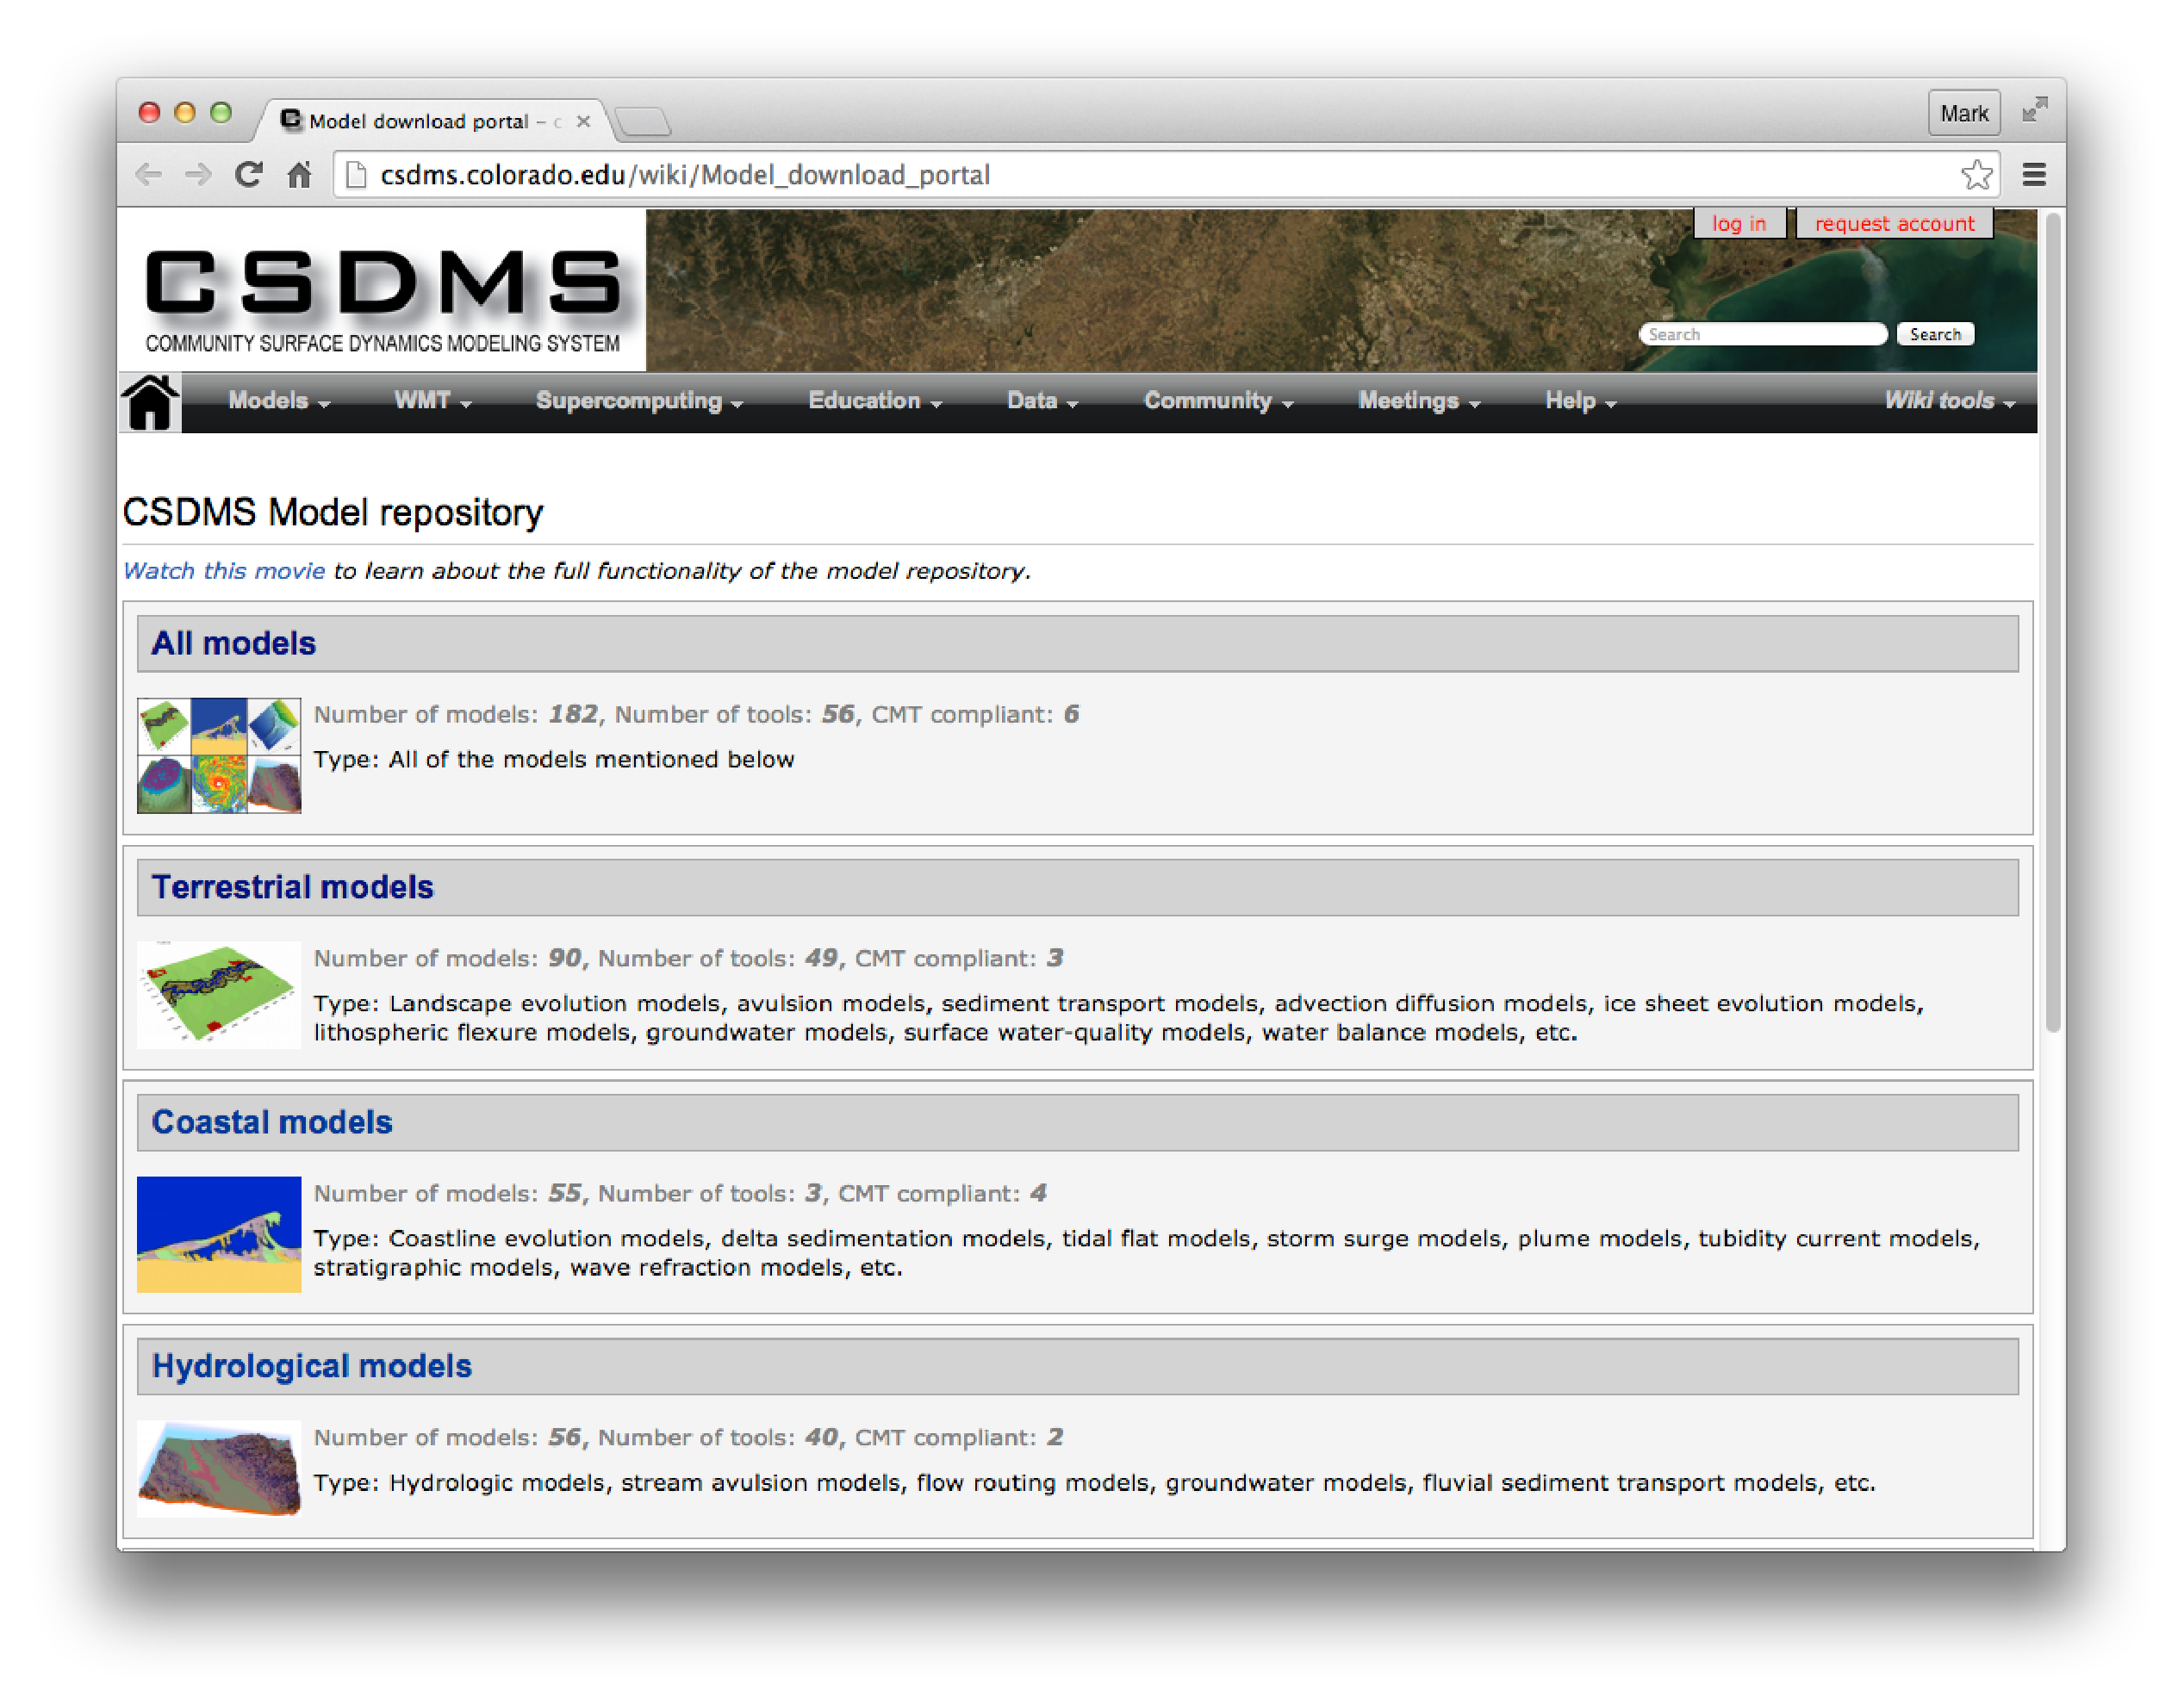
\includegraphics[scale=.25]{csdms_model_repository.eps}
  \end{center}
  \label{fig:model_repository_screenshot}
\end{figure}

\subsection{Digital Object Identifiers for Numerical Models}
\label{sec:doi}

\csdms{} has implemented a
Digital Object Identifier (\doi{}) system for software within its model
repository to guarantee recognition to software contributors.
\csdms{} was among the first software venues to assign \doi{}s to
open source software. The advantages of adopting a \doi{} system for open
source software are: 
\begin{itemize}
\item Guarantee credit to the software developer
\item Easily reuse and replicate research as software is directly locatable 
\item Increase software visibility: \doi{} content is 5 times more likely to
      deliver active links than content without.
\item Provide funding agencies with the ability to track usage, to measure
      impact.
\end{itemize}

Only stable versions of open source
software that are physically hosted through the \csdms{} model repository are
assigned a \doi{}. For model software citations, \csdms{} recommends the
following the DataCite guidelines~\cite{brase2009datacite}.

\begin{shaded}
\leftskip 0.25in
\parindent -0.25in
\tt{
Developer, A., Developer, B. (Year of publication). \emph{Name of the model},
Model Version. Identifier.
}
\end{shaded}

\section{Reusable Components}
\label{sec:reusable}

\subsection{Sustainability and Interoperability Through Standards}
\label{sec:standards}

\subsubsection{The Basic Modeling Interface}
\label{sec:bmi}

The \emph{Basic Modeling Interface}\footnote{https://github.com/csdms/bmi}
(\bmi{}) is a component-coupling library
interface specification designed by \csdms~\cite{peckham2012component,
syvitski2014plug}.  In this context, a component is software that models a
particular environmental process and can be \emph{plugged into} another
component.

The \bmi{} specification was designed without any particular model-coupling
framework in mind.  Rather, it was designed to be framework agnostic. We
recognize model-coupling frameworks and tools may come and go but the
functionality a framework requires from its components will be significantly
more long-lived. Thus, a component should outlive any framework that it might
operate within.

The \bmi{} identifies the entry points into software components that provide a
calling application with the necessary level of control to connect components.
\csdms{}, as well as other modeling frameworks such as
ESMF~\cite{hill2004architecture}, OpenMI~\cite{gregersen2007openmi}, and
OMS~\cite{david2002object}, identifies an interface that, at a minimum,
provides functionality to \emph{initialize}, \emph{update}, and
\emph{finalize} a component. For more complicated (and 2-way)
coupling, components must implement \bmi{} methods providing data access,
and model metadata. For data access, \bmi{} defines a set of \emph{getter}
and \emph{setter} methods that allow model components to present internal data
for both reading and writing.

\csdms{} has found that \bmi{} is an acceptable target for model developers.
The use of \bmi{} has also dramatically reduced the effort required by
\csdms{} staff to create and maintain components. So long as a model component
strictly exposes a \bmi{}, it can automatically be incorporated into the
\csdms{} model-coupling framework where it can then connect to compatible
components to form larger models and obtain additional functionality through
\bmi{} compatible tools (for example, NetCDF output, grid mapping).

\subsubsection{\csdms{} Standard Names}
\label{sec:standardnames}

The \csdms{} \emph{Standard Names}
\footnote{https://github.com/csdms/standard\_names}
are a common language for variable names exchanged between models. They play
an important role in the \bmi{} as they provide a mapping of a model's
internal variable names to a common language used by the \bmi{} getter and
setter functions.

Most models require input variables and produce output variables. For model
components to be reusable and interoperable (either within the \csdms{}
framework or any framework in general)
a set of components become a complete model when every component is able to
obtain the input variables it needs from another component. The \csdms{}
Standard Names were developed to provide a practical solution to this
semantic mediation problem ~\cite{peckham2012component, syvitski2014plug}.
The \csdms{} Standard Names provide a comprehensive set of naming rules and
patterns for creating unique labels for model variables that are not specific
to any particular modeling domain.

\subsection{Connecting and Running Models Through the Web}
\label{sec:wmt}

The \csdms{} Web Modeling Tool\footnote{https://csdms.colorado.edu/wmt}
(\wmt{}) is a web
application that provides an Ajax client-side (the \wmt{}
client\footnote{https://github.com/csdms/wmt-client}) graphical interface
(Figure~\ref{fig:wmt_screenshot}) and a RESTful
server-side database and API (the \wmt{} server\footnote{https://github.com/csdms/wmt})
that allows users to build and run coupled models of earth surface processes on
a high-performance computing cluster from a web browser. \wmt{} was designed
with three objectives:
\begin{itemize}

\item \emph{Accessibility}. As a web-based application, access
      to the Internet implies access to \wmt{}.

\item \emph{Integration}. Easily hyperlink from \wmt{} to resources on the 
      \csdms{} portal (model documentation, labs, lectures,
      tutorials)
      %tutorials and movies - or to other resources on the Internet.

\item \emph{Portability}. \wmt{} has a native JavaScript interface. JavaScript
      is an open standard and almost every computer is equipped with a
      JavaScript-capable web browser.

\end{itemize}

\begin{figure}
  \caption{The \csdms{} Web Modeling Tool}
  \begin{center}
    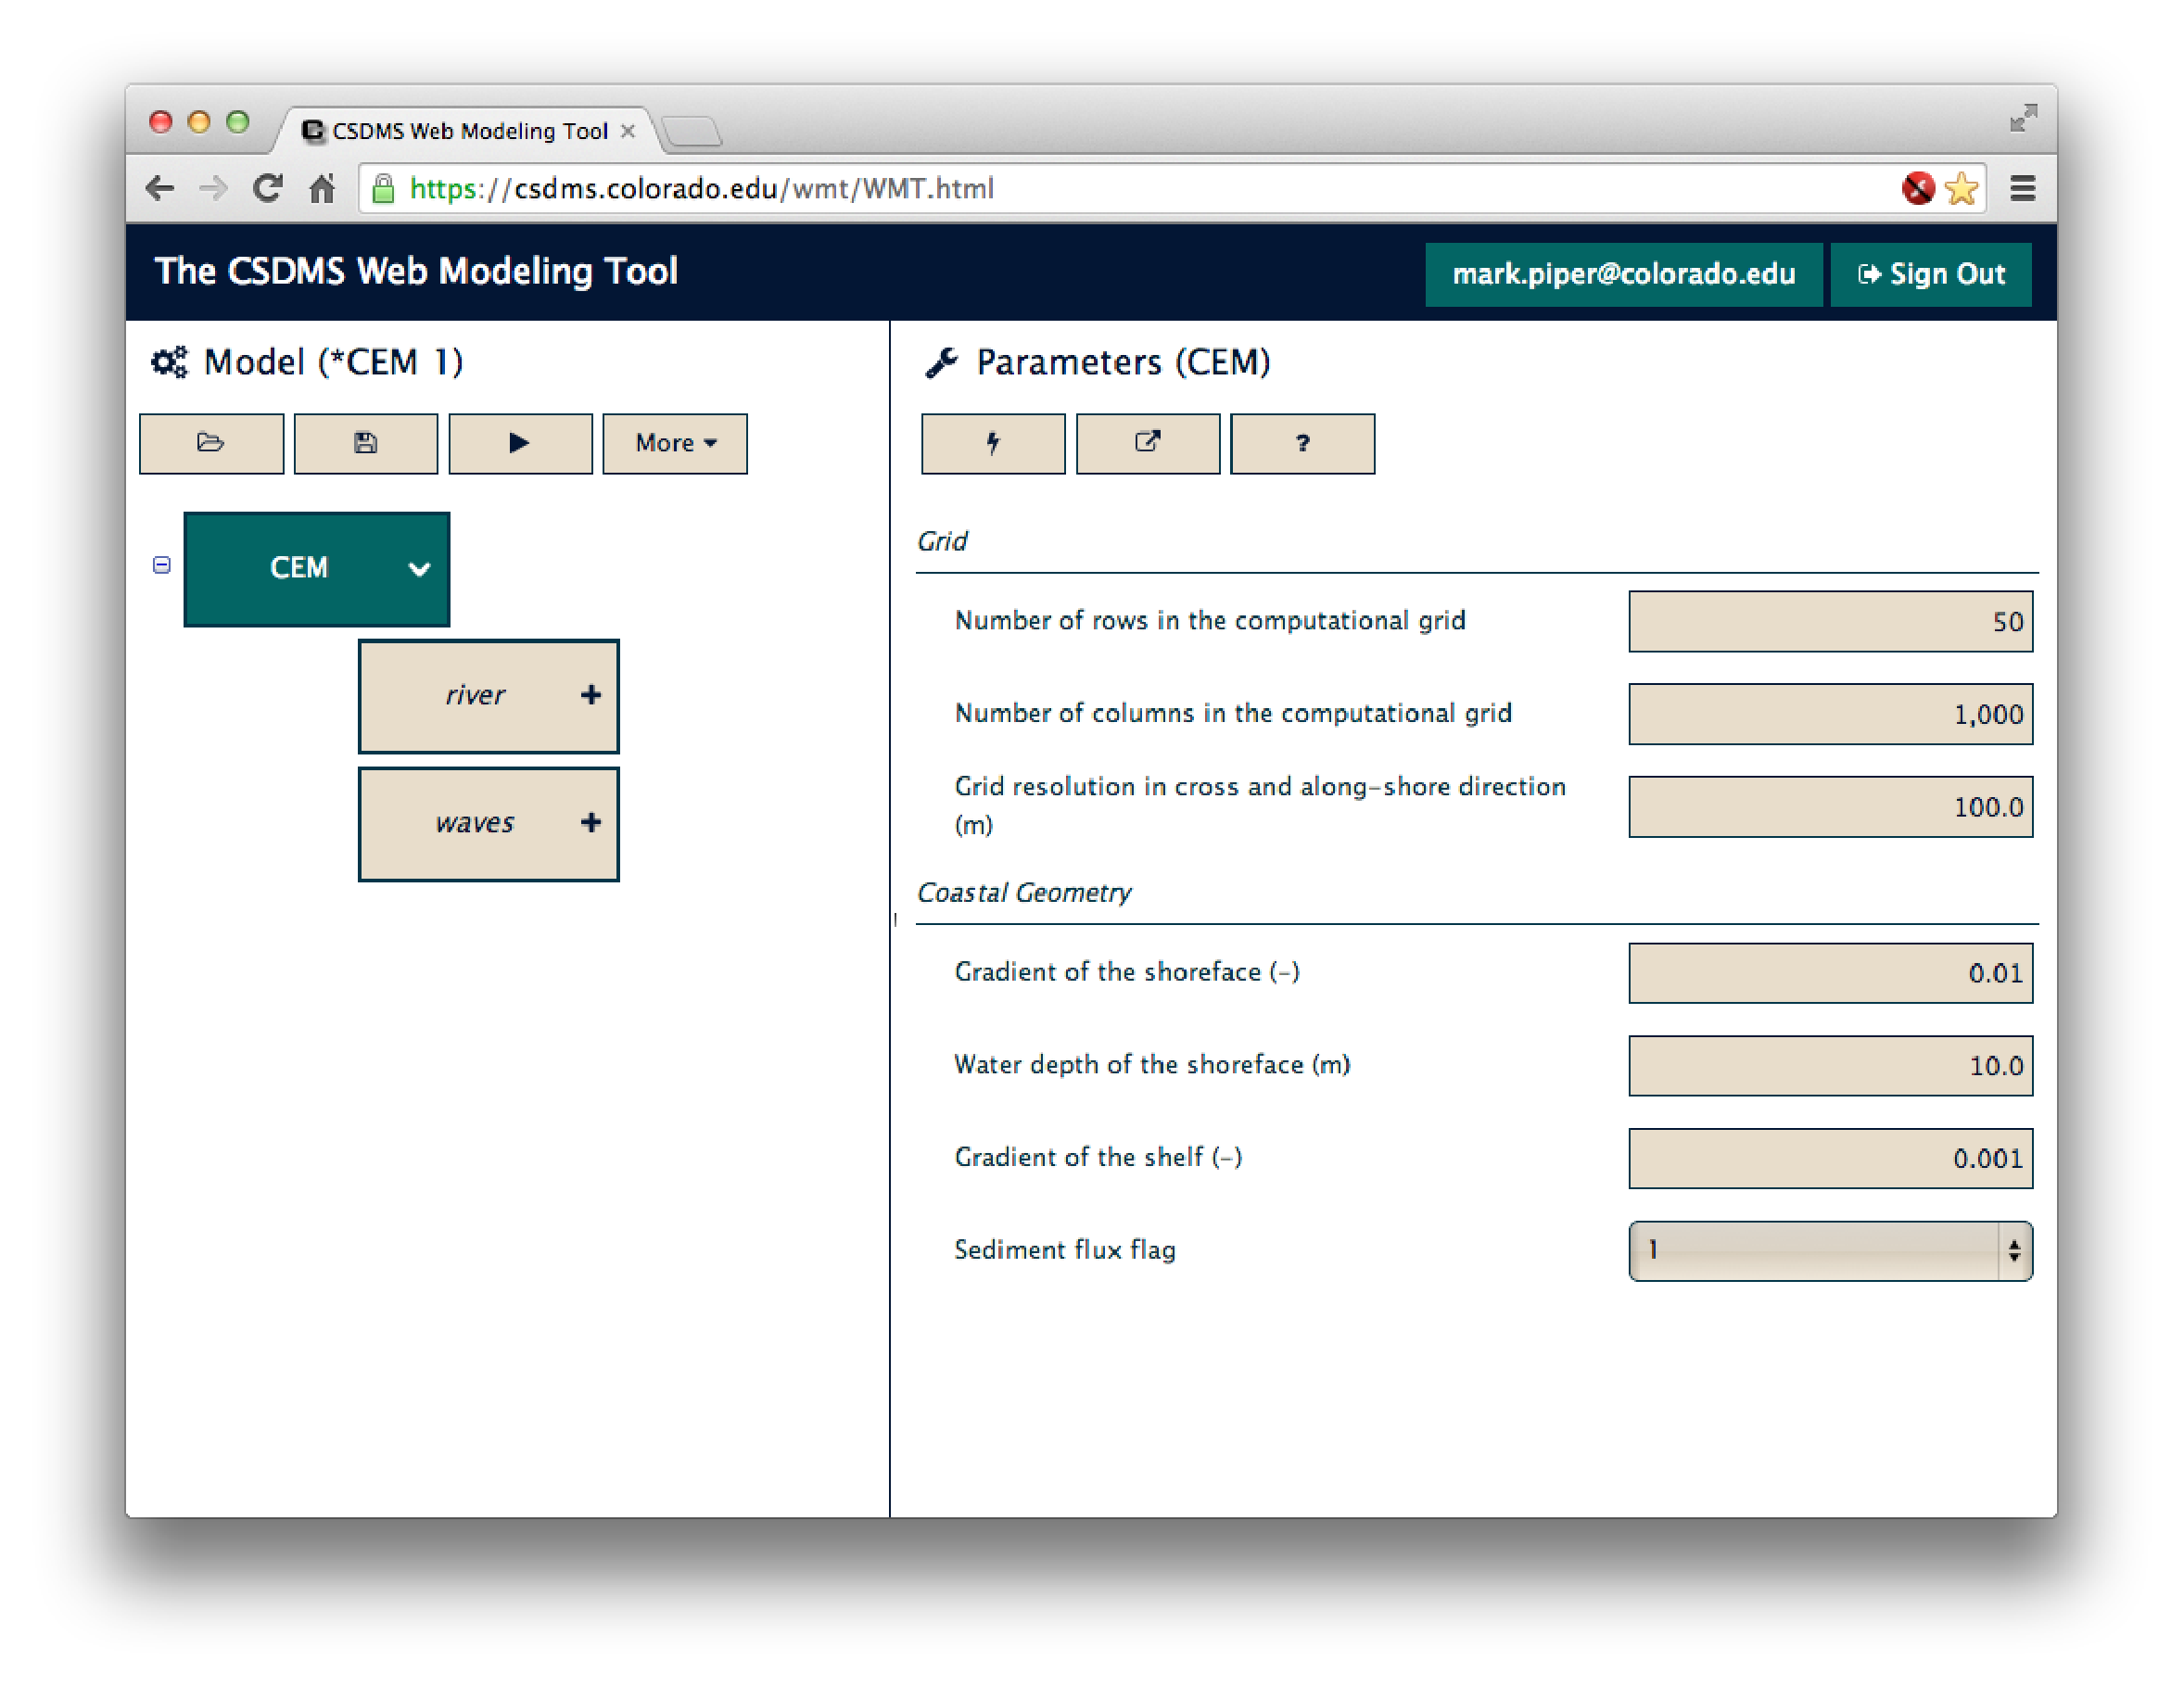
\includegraphics[scale=.25]{wmt.eps}
  \end{center}
  \label{fig:wmt_screenshot}
\end{figure}


With \wmt{}, users can: \emph{run} single component models, build (2-way)
\emph{coupled models}, view and \emph{edit} model parameters, and \emph{share}
saved models with others in the community.

%% \wmt{}, and the software stack on which it is built, are portable.


\begin{comment}
\begin{itemize}

\item select and run a single component model

\item build a coupled model from multiple components

\item view and edit the parameters of the model components;

%\item save models to a server, where they can be accessed on any computer
%      connected to the Internet;

\item share saved models with others in the community;

%\item run a model by connecting to a remote HPCC where the components are
%      installed.

\end{itemize}
\end{comment}

\begin{comment}
\subsection{Software sustainability through expanded functionality}

Another important goal of \csdms{} is to enable the rapid development and application of linked dynamical models tailored to specific landscape-basin evolution problems and at specific temporal and spatial scales. Interdisciplinarity and coupling is a critical step towards advancing predictive modeling~\cite{voinov2010community}.

\csdms{} develops a modeling environment containing a suite of integrated, ever-improving software modules, with expanded functionality beyond the original stand-alone codes. 

The modeling coupling framework is designed to catalyze Earth-surface process research by empowering a broad community of scientists, students and applied modelers with computing tools, streamlining the process of idea generation and hypothesis testing through linked surface dynamics models, and enabling rapid creation and coupling of models tailored to specific settings, scientific problems, and time scales
\end{comment}

\section{Communication and Education}
\label{sec:education}

%\wmt{} provides the ability to run models with an easy to use graphical
%interface and intends to serve novice and more experienced modelers alike.
%The WMT beta version was released in May 2014  as a sequel to the CMT.

\subsection{The CSDMS Portal}

The \csdms{} portal\footnote{http://csdms.colorado.edu}
is the information clearinghouse for the community.
Through the portal,
members can get the latest news,
access model metadata and source code (Section~\ref{sec:organizing}),
view conference and workshop announcements,
view recent job postings,
and access \csdms{} reports, presentations, and publications.
%% including educational presentations and short course
%% materials from \csdms{}-hosted or sponsored workshops.
The portal uses the open-source MediaWiki software,
so \csdms{} members can edit, update and extend existing material,
as well as contribute new material to the portal.

\subsection{User Training}

\csdms{} provides user training in modeling and model coupling
on high-performance computing clusters
through short courses held at 
the University of Colorado,
the International Summer Institute at the University of Minnesota,
and at \csdms{} Annual Meetings.
Course materials are posted to the \csdms{} portal as educational resources.
In addition to training community members,
the clinics also provide an excellent opportunity 
for feedback on using \csdms{} software tools.

\subsection{Programming Courses}

It has been our experience that new graduate students in the Earth
sciences begin with little or no programming experience. However,
their interest in programming is high and they see the importance of
programming with regard to their thesis topics. More often than not,
programming courses are not offered as part of their coursework and
so, out of necessity to solve a particular problem, students end up
teaching themselves how to program.

We believe providing these students with even a small base in programming 
and guidelines on best practices will go a long way. We have
hosted several programming workshops, including one through Software
Carpentry. The workshops were such a success that we are now planning
an annual Software Carpentry bootcamp that is specifically targeted
to incoming graduate students. The workshops fill up nearly
immediately, which reflects a strong interest and need for basic
software skills. We believe these workshops strike a good balance
between teaching students about computer science topics and
maintaining a pragmatic focus on problem solving.

\section{Summary: Building an active and efficient modeling community}

\csdms{} provides cyber-infrastructure to promote the quantitative modeling of
earth surface processes. The US National Science Foundation funds \csdms{}, but
the community is international and includes industry and federal agency
representatives in addition to members from academic institutions. The
initiative has been growing, adding more than 150 people per year. \csdms{} now
fosters a community of over 1200 scientists who work on determining
the movement of fluids, and the production, erosion, transport, and
deposition of sediment and nutrients in landscapes and seascapes. 

\section{Acknowledgements}

The \csdms{} Integration Facility operates under continuing grant 0621695
from the US National Science Foundation.

\bibliographystyle{plain}

\bibliography{article-citations}{}

\end{document}
